\subsection{Label Bias}
\begin{figure}[h!]
    \centering
    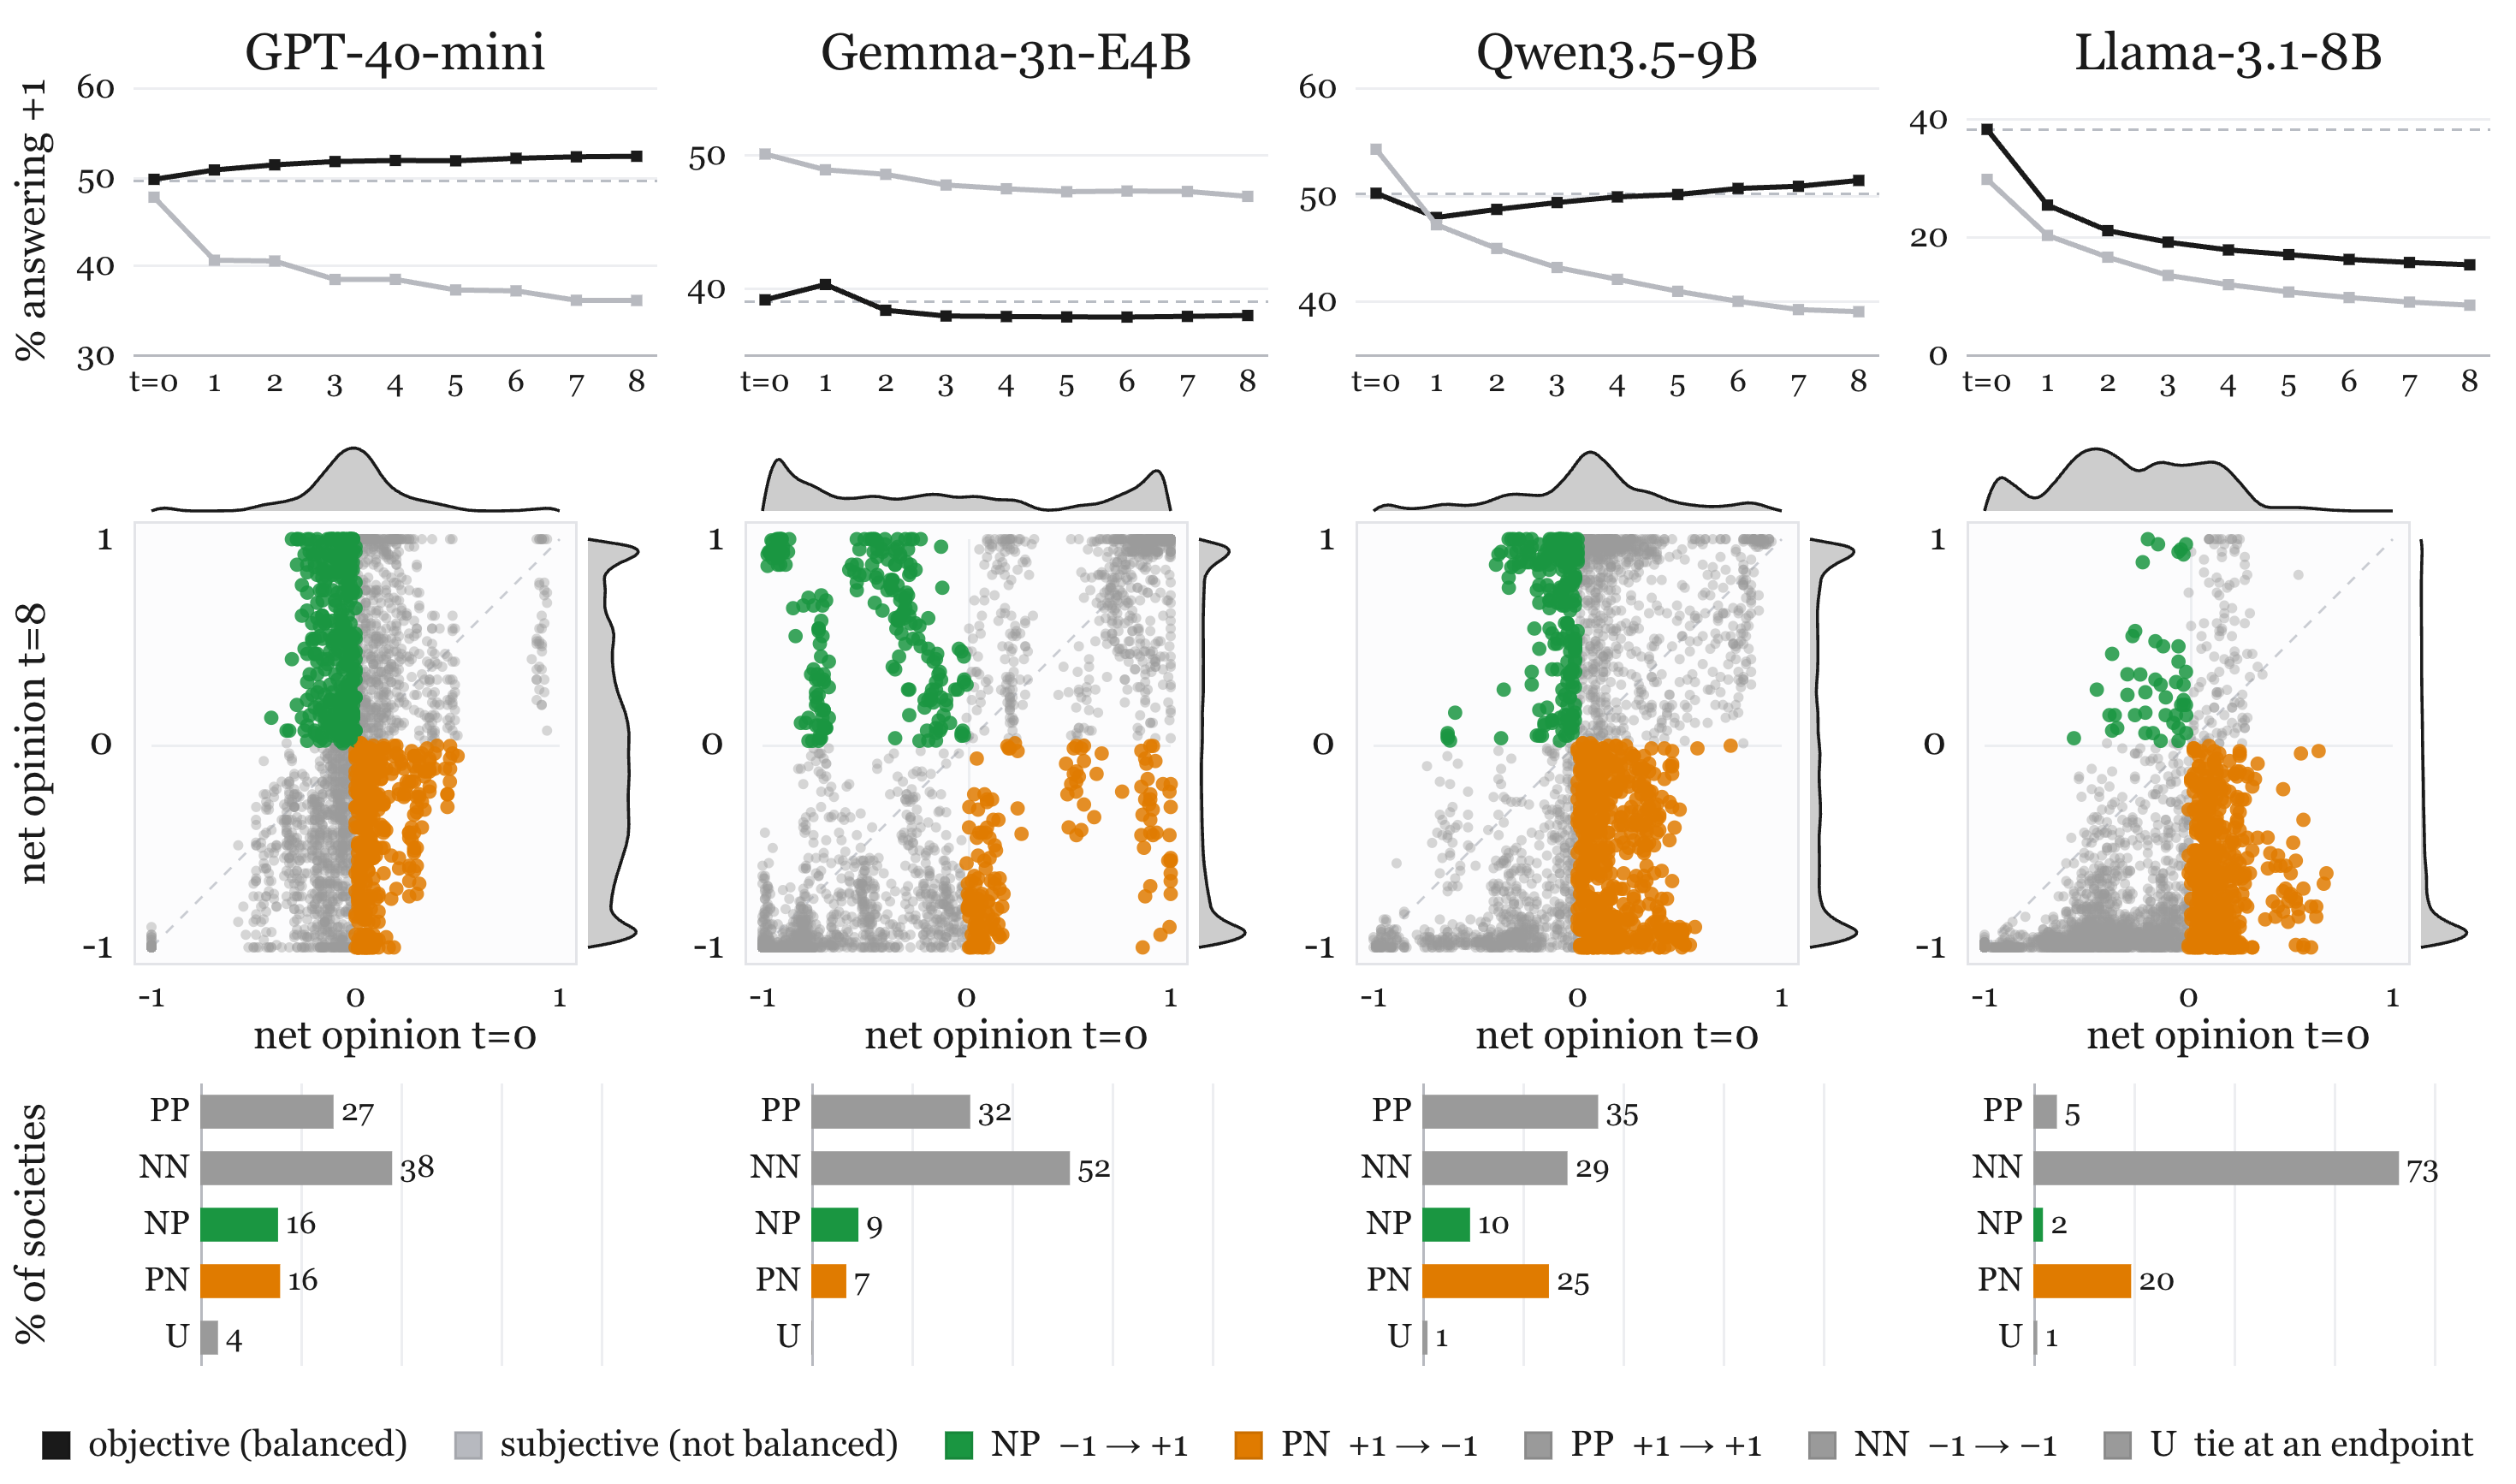
\includegraphics[width=0.99\textwidth]{main/Figures/apx_05_label_bias.png}
            \caption{\textit{Label Bias.} How opinions move along the $+1 / -1$ axis over the run ($9,600$ groups from both objective and subjective questions, spanning signed random graphs and the square and triangular lattices, over both the training- and test-set questions). \emph{Row 1:} $y$-axis: percentage of group trajectories, where the net opinion $n(t)$ has positive sign at round $t$. $x$-axis: timesteps. \emph{Row 2:} Each point represents a group trajectory, which is plotted based on its initial ($t=0$, $x$-axis) and final ($t=8$, $y$-axis) net opinion $n(t)$  \emph{Row 3:} Groups switch between $+1$ and $-1$ at $t=0$ and $t=8$. PP (positive$\to$positive), NN (negative$\to$negative), NP (negative$\to$positive), PN (positive$\to$negative), and U (undecided, $50\text{-}50$ tie at $t=0$ or $t=8$). The two transition categories NP and PN are highlighted.}
\label{fig:3_Observations_bias}
\end{figure}

\textit{Label Bias.} A community can also drift toward an answer option irrespective of what that option says (Figure~\ref{fig:3_Observations_bias}). Because the objective questions are label balanced, with the correct answer being $+1$ as often as $-1$, a change in the fraction of agents answering $+1$ over the course of a run cannot be attributed to truth seeking. However, we still observe such a change for Llama-3.1-8B-Instruct, with the fraction answering $+1$ falling from $39\%$ to $16\%$.
